%Notes by Harsh Mistry 
%Econ 301
%Based on Template From  https://www.cs.cmu.edu/~ggordon/10725-F12/template.tex

\documentclass[twoside]{article}
\setlength{\oddsidemargin}{0.25 in}
\setlength{\evensidemargin}{-0.25 in}
\setlength{\topmargin}{-0.6 in}
\setlength{\textwidth}{6.5 in}
\setlength{\textheight}{8.5 in}
\setlength{\headsep}{0.75 in}
\setlength{\parindent}{0 in}
\setlength{\parskip}{0.1 in}
\usepackage{amsmath,amsfonts,graphicx, color}
\newcounter{lecnum}
\renewcommand{\thepage}{\thelecnum-\arabic{page}}
\renewcommand{\thesection}{\thelecnum.\arabic{section}}
\renewcommand{\theequation}{\thelecnum.\arabic{equation}}
\renewcommand{\thefigure}{\thelecnum.\arabic{figure}}
\renewcommand{\thetable}{\thelecnum.\arabic{table}}
\newcommand{\lecture}[4]{
   \pagestyle{myheadings}
   \thispagestyle{plain}
   \newpage
   \setcounter{lecnum}{#1}
   \setcounter{page}{1}
   
   
%Info Box 
   \begin{center}
   \framebox{
      \vbox{\vspace{2mm}
    \hbox to 6.28in { {\bf Econ 301 - Microeconomic Theory 2
	\hfill Winter 2018} }
       \vspace{4mm}
       \hbox to 6.28in { {\Large \hfill Lecture #1: #2  \hfill} }
       \vspace{2mm}
       \hbox to 6.28in { {\it Lecturer: #3 \hfill Notes By: #4} }
      \vspace{2mm}}
   }
   \end{center}
   
   \markboth{Lecture #1: #2}{Lecture #1: #2}



 
}

\renewcommand{\cite}[1]{[#1]}
\def\beginrefs{\begin{list}%
        {[\arabic{equation}]}{\usecounter{equation}
         \setlength{\leftmargin}{2.0truecm}\setlength{\labelsep}{0.4truecm}%
         \setlength{\labelwidth}{1.6truecm}}}
\def\endrefs{\end{list}}
\def\bibentry#1{\item[\hbox{[#1]}]}

\newcommand{\fig}[3]{
			\vspace{#2}
			\begin{center}
			Figure \thelecnum.#1:~#3
			\end{center}
	}
	
	\graphicspath{ {images/} }

\newtheorem{theorem}{Theorem}[lecnum]
\newtheorem{lemma}[theorem]{Lemma}
\newtheorem{ex}[theorem]{Example}
\newtheorem{proposition}[theorem]{Proposition}
\newtheorem{claim}[theorem]{Claim}
\newtheorem{corollary}[theorem]{Corollary}
\newtheorem{definition}[theorem]{Definition}
\newenvironment{proof}{{\bf Proof:}}{\hfill\rule{2mm}{2mm}}
\newcommand\E{\mathbb{E}}


%Start of Document 
\begin{document}

\lecture{15}{March 7, 2018}{Jean Guillaume Forand}{Harsh Mistry}

\section{Welfare Continued}

\subsection{Second Welfare Theorem}
\textcolor{red}{In-Class Numbering : 3.2} 
\begin{itemize}
\item We may have reasons to prefer some Pareto-efficient allocations over others. 
\item Does this limit the importance of the first welfare theorem? (i.e do competitive equilibriums always yield "bad" or "unfair" Pareto-efficient allocations)
\item To be concrete : we shall define what it means for an allocation to be \underline{fair}
\item \textbf{First Attempt :} say allocations \(x^A\) and \(x^B\) are \underline{fair} if \(x_i^A = x_i^B\) for all \(i = 1, 2\) 
\begin{center}
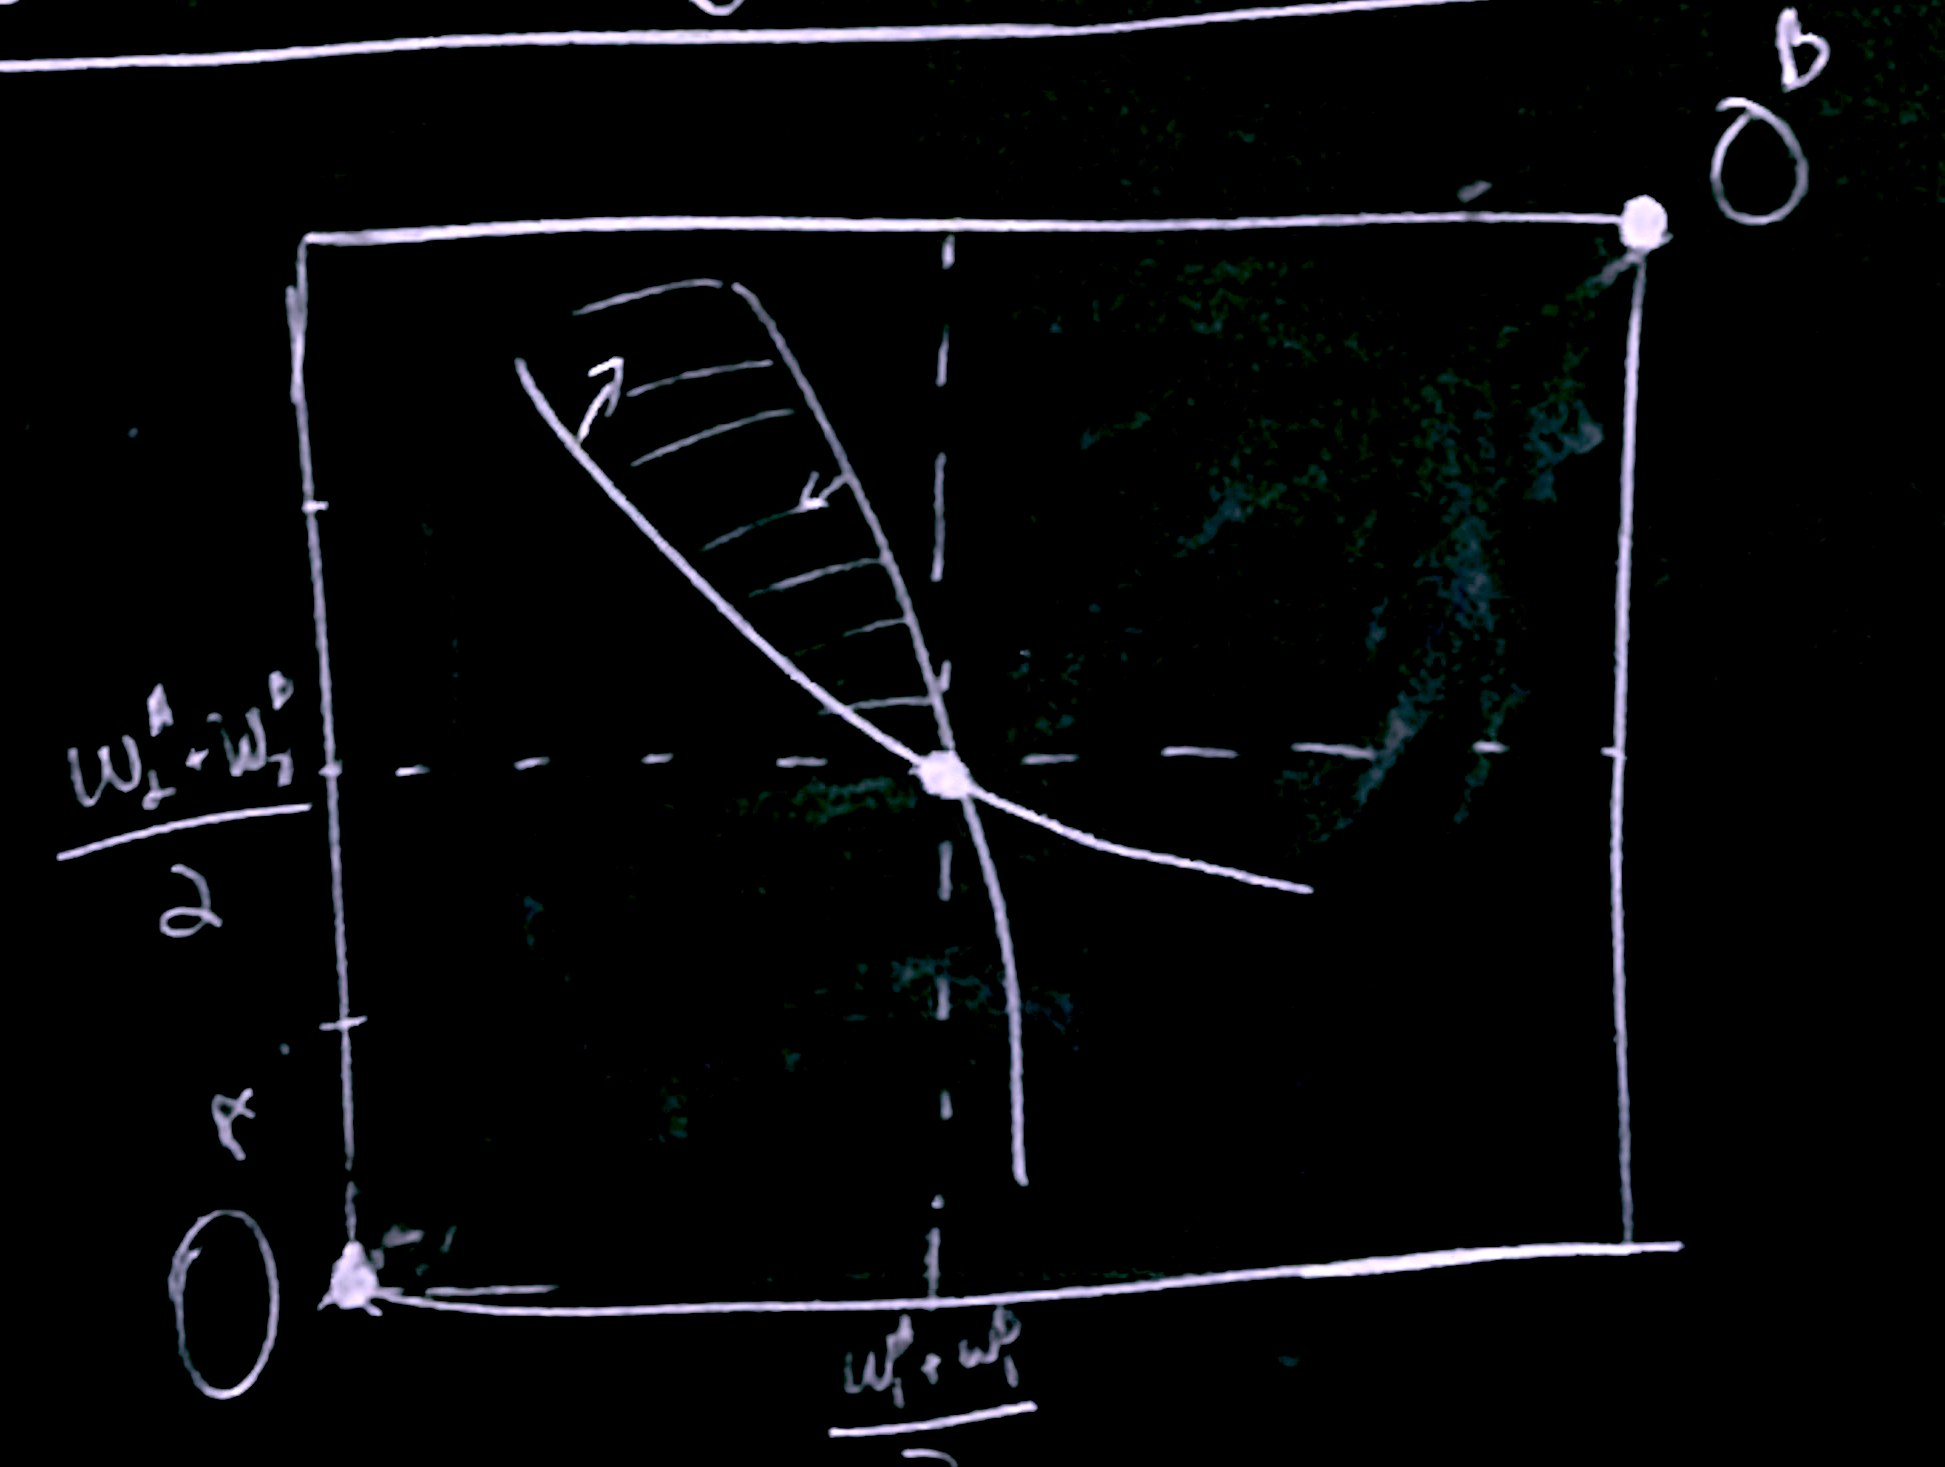
\includegraphics[scale=0.07]{27}
\end{center}
\begin{itemize}
\item These fair allocations are not generally Pareto-efficient, thus this  really isn't a useful definition of fairness. 
\end{itemize}
\item Pareto-efficiency is minimal normative criterion, we want a definition of fairness that selects among these.
\end{itemize}
\begin{definition} Allocations \(x^A\) and \(x^B\) have \underline{no envy} if \(u^A(x_1^A, x_2^B) \geq u^A(x_1^B, x_2^B\) and 
\(u^B(x_1^A, x_2^A) \geq u^B(x_1^A, x_2^A)\)
\end{definition}
\begin{definition}
Allocations \(x^A\) and \(x^B\) are \underline{fair} if they are Pareto-efficient and satisfy no-envy. 
\end{definition}
\begin{itemize}
\item How to calculate fair allocations?
\begin{enumerate}
\item Start with equal-division allocation.
\item If it is pareto-efficient, then its fair.
\item If equal division is not pareto-efficient, 
\begin{itemize}
\item Fix any allocations \(x^A, x^B\) that are PE and Pareto dominate equal-division.
\item Result : If consumers preferences are monotone and convex, then allocations \(x^A\) and \(x^B\) are fair. 
\begin{center}
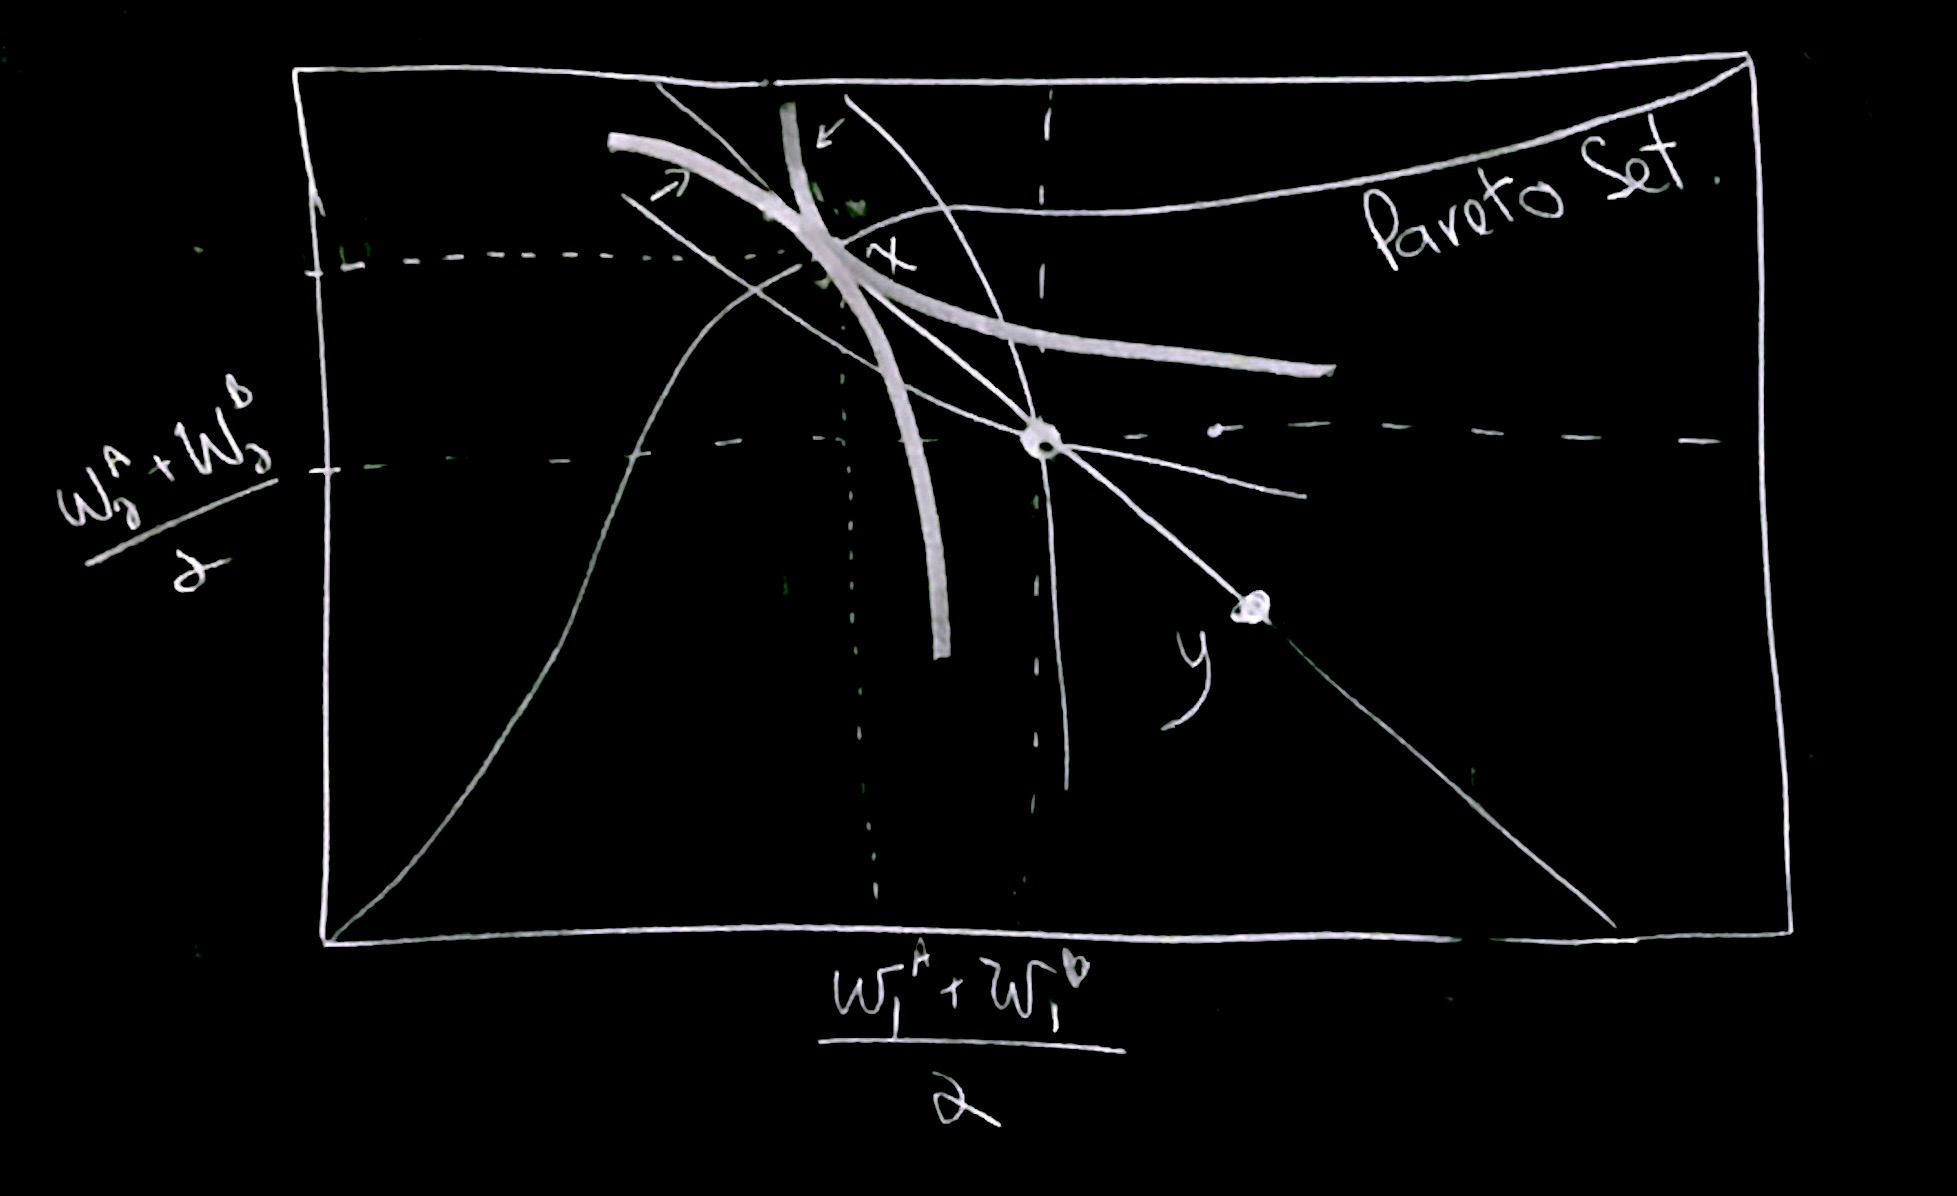
\includegraphics[scale=0.1]{28}
\end{center}
\item Say allocations \(y^A, y^B\) are such that \(y^A = y^B\)and \(y^B = x^A\)
\item In the figure, these allocations lie on the line through x and equal-division allocation
\item So, we have \(U^J(y^J_1, y^J_2) \leq u^J(x_1^J, x_2^J)\) for \(J=A, B\)
\end{itemize}
\end{enumerate}
\end{itemize}





\end{document}





